\chapter{Spanning Tree Protocol (STP)}

\section{Home Preparation}

\begin{center}
\sffamily\small
\begin{tabular}{>{\columncolor{tablegray}}p{15cm}}
\multicolumn{1}{>{\columncolor{tablered}}l}{Important}\\
For this practical exercise, you have to submit a report the answers to the questions below. When submitting the answers to the questions, be brief but precise. If you include screenshots, indicate on the screenshot what is the answer.\\
\hline
\end{tabular}
\end{center}

The user manual for the switch is available here:

\url{http://www.jaumebarcelo.info/teaching/lxs/stp/manual_spantree.pdf}

\section{Introduction}

In this assignment you will configure the Spanning Tree Protocol (STP). This protocol is used in Ethernet networks to establish which are the active link and therefore which is the path that data packets will follow. The switches that you will use are the same as the ones in the previous assignment. Have your VLAN report handy just in case you need to consult it and to remember which are the basic commands to interact with the switch.

\section{Theoretical Construction of the Tree}

The switches are connected as illustrated in the figure \ref{fig:StpTopology}.

\begin{figure}
\centering
\ifpdf
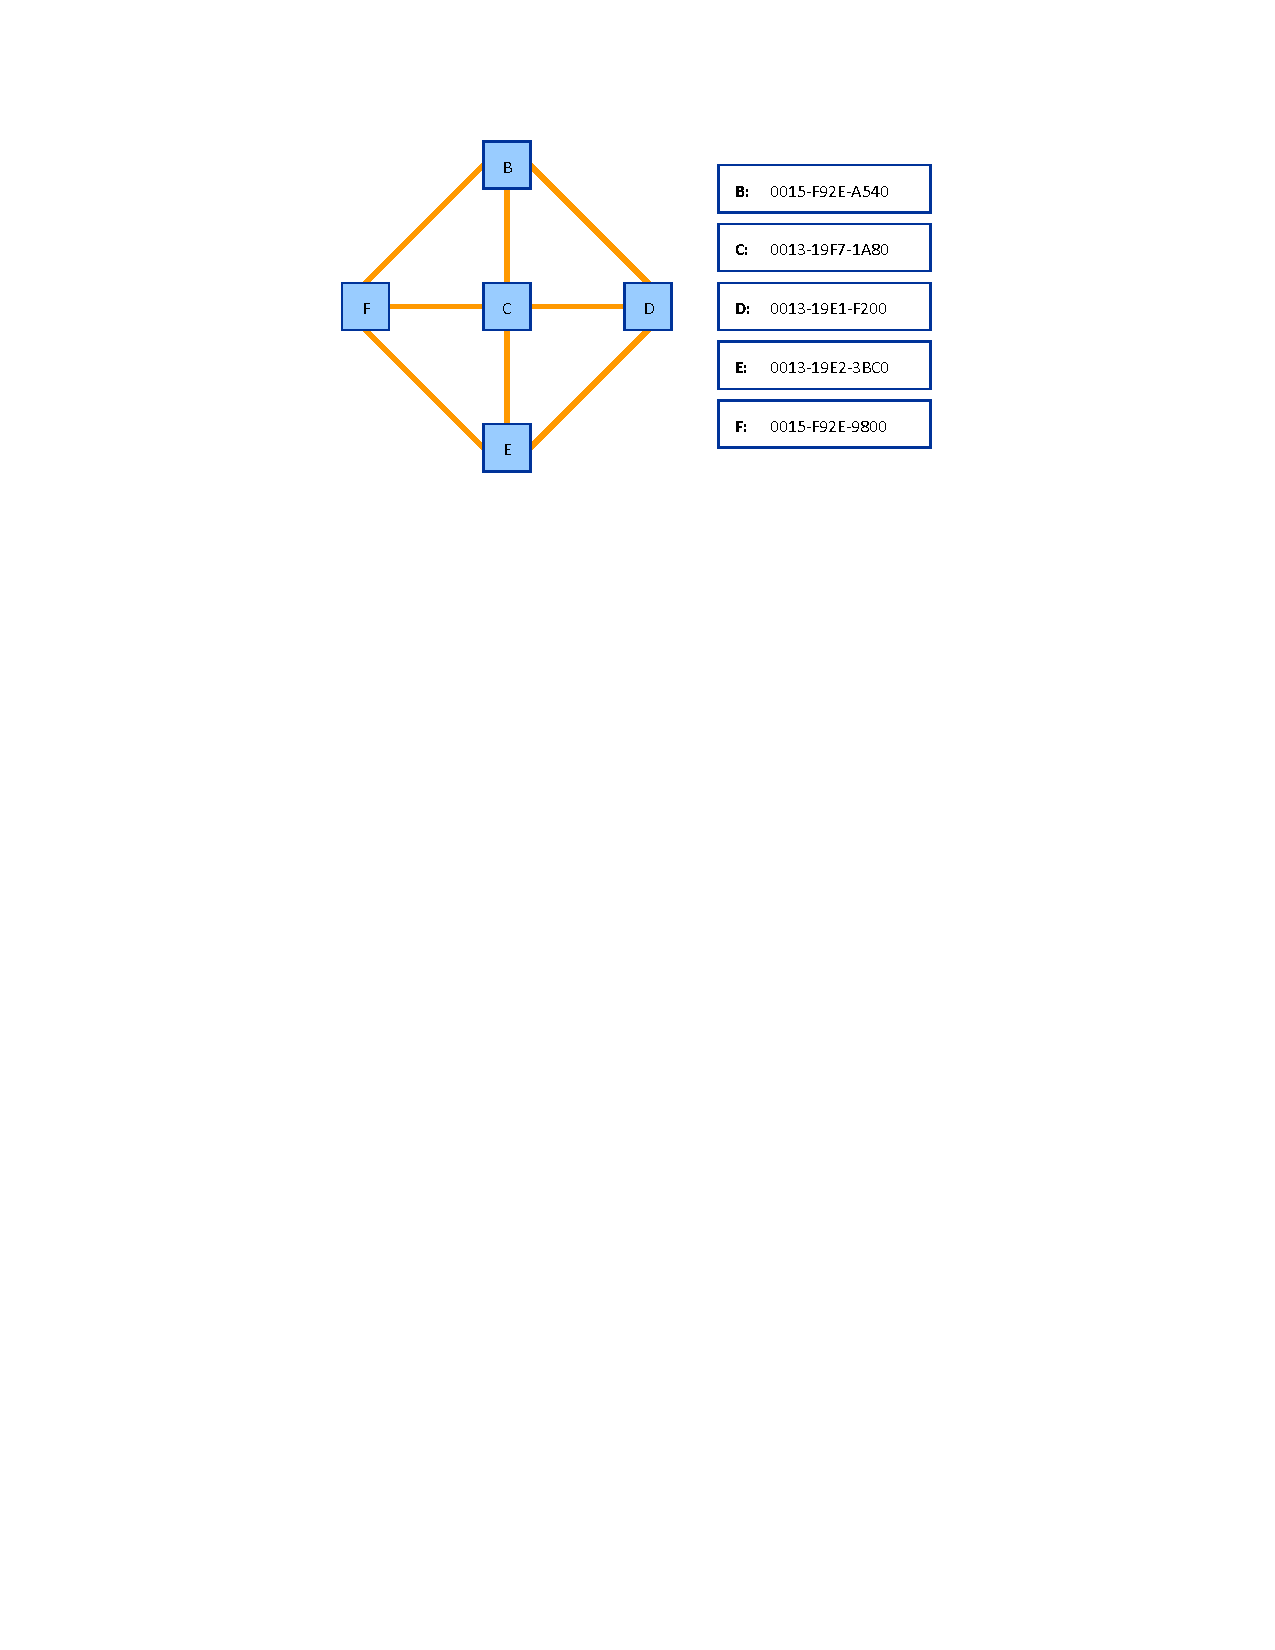
\includegraphics[width=0.9\linewidth]{Figures/StpTopology.pdf}
\else
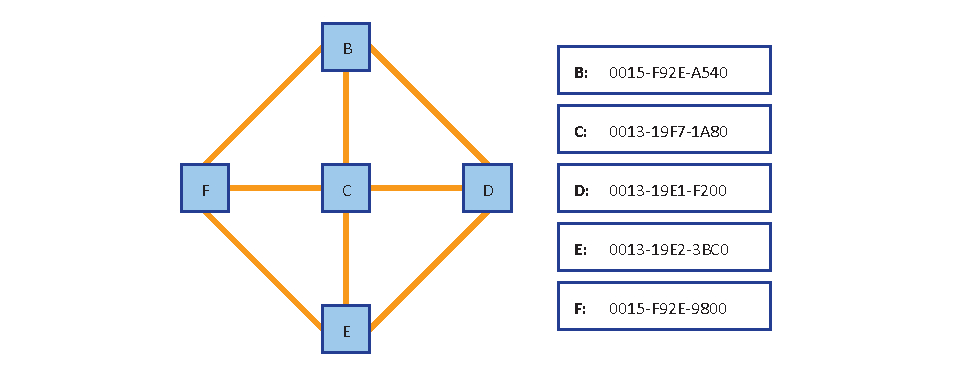
\includegraphics[width=0.9\linewidth]{Figures/StpTopology.eps}
\fi
\caption{The network topology used for the STP practical exercise.}
\label{fig:StpTopology}
\end{figure}

\begin{center}
\sffamily\small
\begin{tabular}{>{\columncolor{tablegray}}p{15cm}}

\multicolumn{1}{>{\columncolor{tableorange}}l}{Questions and Tasks}\\
If the priority is \texttt{\color{blue}32768} (\texttt{\color{blue}0x8000}), what is the \texttt{\color{blue}Bridge ID} of each switch? \textbf{(5\,\%)}\\
\hline
Which is the root switch? \textbf{(5\,\%)}\\
\hline
Compute which is the spanning tree and draw it. \textbf{(10\,\%)}\\
\hline
Fill in the table \ref{tab:Stp}, indicating for each switch the role and state of each trunk port. \textbf{(10\,\%)}\\
\hline
\end{tabular}
\end{center}

\begin{table}
\sffamily\small
\centering
\begin{tabular}{>{\columncolor{tablegray}}cccccc}
\multicolumn{1}{>{\columncolor{tableorange}}c}{Switch name} & \multicolumn{1}{>{\columncolor{tableheader}}c}{MAC} & \multicolumn{1}{>{\columncolor{tableheader}}c}{Bridge ID} & \multicolumn{1}{>{\columncolor{tableheader}}c}{Port} & \multicolumn{1}{>{\columncolor{tableheader}}c}{Role} & \multicolumn{1}{>{\columncolor{tableheader}}c}{State} \\
Switch B & 00:15:F9:2E:A5:40 & {\color{red}?} & {\color{red}?} & {\color{red}?} & {\color{red}?} \\
\hline
Switch C & 00:13:19:F7:1A:80 & {\color{red}?} & {\color{red}?} & {\color{red}?} & {\color{red}?} \\
\hline
Switch D & 00:13:19:E1:F2:00 & {\color{red}?} & {\color{red}?} & {\color{red}?} & {\color{red}?} \\
\hline
Switch E & 00:13:19:E2:3B:C0 & {\color{red}?} & {\color{red}?} & {\color{red}?} & {\color{red}?} \\
\hline
Switch F & 00:15:F9:2E:98:00 & {\color{red}?} & {\color{red}?} & {\color{red}?} & {\color{red}?} \\
\hline
\end{tabular}
\caption{The spanning tree.}
\label{tab:Stp}
\end{table}

\section{Practical Verification}

Now you will verify that the STP constructed by the switches is in fact the one you computed in the previous section. Use the VLAN 1 to connect to the five switches (B, C, D, E, F). It is recommended to open five simultaneous Telnet connections, one for each of the switch.

Each group will work in a different VLAN. The teacher will assign a VLAN to each group. Make sure that your VLAN is included in all the trunk ports. Each group will have a different STP, as the network creates a tree for each VLAN.

In each of the switches, enter the \emph{privileged EXEC} mode and use the command:

\begin{lstlisting}
Switch# show spanning-tree vlan <id>
\end{lstlisting}

Observe all the fields and make sure you understand them.

\begin{center}
\sffamily\small
\begin{tabular}{>{\columncolor{tablegray}}p{15cm}}
\multicolumn{1}{>{\columncolor{tableorange}}l}{Questions and Tasks}\\
What is the \texttt{\color{blue}Bridge ID} of each switch? Indicate the MAC and the priority. \textbf{(5\,\%)}\\
\hline
For the \texttt{\color{blue}Bridge ID} priority of each switch, what is the base priority value set by the switch administrator? \textbf{(5\,\%)}\\
\hline
Compute which is the spanning tree and draw it. \textbf{(5\,\%)}\\
\hline
Fill in the table \ref{tab:Stp}, indicating for each switch the role and state of each trunk port. Are the theoretical and practical results identical? \textbf{(5\,\%)}\\
\hline
\end{tabular}
\end{center}

\section{Changing the STP Configuration}

Now that you are familiar with the STP parameters, you will make some changes that will result in the computation of a new tree. In the \emph{global configuration} mode use the command:

\begin{lstlisting}
Switch(config)# spanning-tree vlan <id>
\end{lstlisting}
or, alternatively, you may use:

\begin{lstlisting}
Switch(config)# interface vlan <id>
Switch(config)# spanning-tree
\end{lstlisting}
to see which parameters are susceptible to be configured. Use the question mark \texttt{\color{blue}?} to see all the available parameters and make sure you understand them.

The exercise that we propose is to change the priority of one of the switches different from the root switch. The default behavior is that the switch with the lowest MAC address is selected as a root. The reason is that, in the default configuration, the priority of all the switches is \texttt{\color{blue}32768} (\texttt{\color{blue}0x8000}). By changing the priority of one of the switches to a lower value, we can force that that particular switch becomes the root.

Change the priority for the root switch and observe the new configuration of the tree.

\begin{center}
\sffamily\small
\begin{tabular}{>{\columncolor{tablegray}}p{15cm}}
\multicolumn{1}{>{\columncolor{tableorange}}l}{Questions and Tasks}\\
Compute which is the new spanning tree and draw it. You must indicate the new priority you assigned to the previous root switch. \textbf{(10\,\%)}\\
\hline
Fill in the table \ref{tab:Stp}, indicating for each switch the role and state of each trunk port. \textbf{(10\,\%)}\\
\hline
\end{tabular}
\end{center}

\section{Link Failure}

\begin{center}
\sffamily\small
\begin{tabular}{>{\columncolor{tablegray}}p{15cm}}
\multicolumn{1}{>{\columncolor{tablered}}l}{Important}\\
For this assignment you must wait until all the groups have finished the previous one. If you reach this exercise before the other groups, move on to the next exercise while you wait for all the groups to be ready for the link failure.\\
\hline
\end{tabular}
\end{center}

Now we will disconnect one of the links to simulate a link failure. Compute in advance your new spanning tree after the link failure. Ask your teacher which is the cable that will be disconnected. After the disconnection, check which is the new configuration and compare it with the one that you have predicted.

\begin{center}
\sffamily\small
\begin{tabular}{>{\columncolor{tablegray}}p{15cm}}
\multicolumn{1}{>{\columncolor{tableorange}}l}{Questions and Tasks}\\
Compute which is the new spanning tree and draw it. You must indicate the link that failed. \textbf{(10\,\%)}\\
\hline
Fill in the table \ref{tab:Stp}, indicating for each switch the role and state of each trunk port. \textbf{(10\,\%)}\\
\hline
\end{tabular}
\end{center}

\section{BPDUs}

Use the computer connected to the VLAN 1 (the computer used for the administration of the switch) and capture the traffic for several seconds using \emph{Wireshark}. Observed the received STP frames and identify the different fields in the packet.

\begin{center}
\sffamily\small
\begin{tabular}{>{\columncolor{tablegray}}p{15cm}}
\multicolumn{1}{>{\columncolor{tableorange}}l}{Questions and Tasks}\\
Include in your report one received STP BPDU, and indicate what the information from the main fields. \emph{Tip: Use the lecture notes to identify the relevant fields.} \textbf{(10\,\%)}\\
\hline
\end{tabular}
\end{center}
